% $Header: /Users/joseph/Documents/LaTeX/beamer/solutions/generic-talks/generic-ornate-15min-45min.en.tex,v 90e850259b8b 2007/01/28 20:48:30 tantau $

\documentclass{beamer}

% This file is a solution template for:

% - Giving a talk on some subject.
% - The talk is between 15min and 45min long.
% - Style is ornate.

\usepackage{graphicx,color,psfrag}
\usepackage{epstopdf}
% Copyright 2004 by Till Tantau <tantau@users.sourceforge.net>.
%
% In principle, this file can be redistributed and/or modified under
% the terms of the GNU Public License, version 2.
%
% However, this file is supposed to be a template to be modified
% for your own needs. For this reason, if you use this file as a
% template and not specifically distribute it as part of a another
% package/program, I grant the extra permission to freely copy and
% modify this file as you see fit and even to delete this copyright
% notice. 


\mode<presentation>
{
  \usetheme{Warsaw}
  % or ...

  \setbeamercovered{transparent}
  % or whatever (possibly just delete it)
}


\usepackage[english]{babel}
% or whatever

\usepackage[latin1]{inputenc}
% or whatever

\usepackage{times}
\usepackage[T1]{fontenc}
% Or whatever. Note that the encoding and the font should match. If T1
% does not look nice, try deleting the line with the fontenc.


\title[Statistical Methods in Fast Fracture of Ceramics] % (optional, use only with long paper titles)
{Statistical Methods in Fast Fracture of Ceramics}

%\subtitle
%{Presentation Subtitle} % (optional)

\author[Burak ER] % (optional, use only with lots of authors)
{Burak ER\inst{1}}
% - Use the \inst{?} command only if the authors have different
%   affiliation.

\institute[Universities of Somewhere and Elsewhere] % (optional, but mostly needed)
{
  \inst{1}%
  Department of Mechanical Engineering\\
  Bursa Technical University
}
% - Use the \inst command only if there are several affiliations.
% - Keep it simple, no one is interested in your street address.

\date[Short Occasion] % (optional)
{30.12.2013 / Fracture Mechanics Class Fall 2013}

\subject{Talks}
% This is only inserted into the PDF information catalog. Can be left
% out. 



% If you have a file called "university-logo-filename.xxx", where xxx
% is a graphic format that can be processed by latex or pdflatex,
% resp., then you can add a logo as follows:

% \pgfdeclareimage[height=0.5cm]{university-logo}{university-logo-filename}
% \logo{\pgfuseimage{university-logo}}



% Delete this, if you do not want the table of contents to pop up at
% the beginning of each subsection:
\AtBeginSubsection[]
{
  \begin{frame}<beamer>{Outline}
    \tableofcontents[currentsection,currentsubsection]
  \end{frame}
}


% If you wish to uncover everything in a step-wise fashion, uncomment
% the following command: 

%\beamerdefaultoverlayspecification{<+->}


\begin{document}

\begin{frame}
  \titlepage
\end{frame}

\begin{frame}{Outline}
  \tableofcontents
  % You might wish to add the option [pausesections]
\end{frame}


% Since this a solution template for a generic talk, very little can
% be said about how it should be structured. However, the talk length
% of between 15min and 45min and the theme suggest that you stick to
% the following rules:  

% - Exactly two or three sections (other than the summary).
% - At *most* three subsections per section.
% - Talk about 30s to 2min per frame. So there should be between about
%   15 and 30 frames, all told.

\section{Introduction}
\subsection[Why Statistical Fracture Analysis fo Ceramics?]{Why Statistical Fracture Analysis fo Ceramics?}
\begin{frame}{Indeterminism of the fracture of ceramic materials}{}
\begin{itemize}
\item {Ceramic is brittle.}
\item {Identical specimens of a ceramic material may exhibit large variations in
fracture stress.}
\item {Strength of brittle material depends on the volume.}
\end{itemize} 
\end{frame}

\begin{frame}{Indeterminism of the fracture of brittle materials}{}
Fracture mechanics view:
\begin{itemize}
\item {Many flaws}
\item {Random flaw size and orientation.}
\end{itemize} 
\end{frame}
\subsection[Key Contributions]{Key Contributions}

\begin{frame}{Key contributions}{Key contributions}
\begin{itemize}
\item{Walladi Weibull 1939,\\"A Statistical Theory of The Strength of Materials."}
\item<1->{Batdorf 1974,\\"A Statistical Theory for the Fracture of Brittle Structures Subjected to Nonuniform Polyaxial Stresses"}
\end{itemize} 
\end{frame}

\begin{frame}{Summary}{Summary}
\begin{itemize}
\item Weibull Theory
    \begin{itemize}
	\item Weakest link theory.
	\item Considers only the uniaxial stress.
	\item Pure statistical
	\end{itemize}
\item<2-> Batdorf
 \begin{itemize}
	\item Multiaxial stress addition to Weibull Theory.
	\item Linear Elastic Fracture Mechanics
\end{itemize}
\end{itemize} 
\end{frame}

\subsection[Fundamental Basis for The Weibull Theory]{Fundamental Basis for The Weibull Theory}
\begin{frame}{Derivation of Weibull's Relation}{Derivation of Weibull's Equation}
Probability of failure of an individual volume element:
\begin{eqnarray*}
(1-P)=(1-P_0)^V
\end{eqnarray*}
\begin{eqnarray*}
ln(1-P)=V ln(1-P_0)\Longrightarrow \text{risk of rupture} \ B
\end{eqnarray*}
\end{frame}
\begin{frame}{Derivation of Weibull's Relation}{Derivation of Weibull's Equation}
Probability of failure = $1-e^B$=$1-e^{\int_{V} N\left(\sigma\right)dV}$
\begin{eqnarray*}
\int_{V} N\left(\sigma\right)dV=-\frac{V}{V_0}\left(\frac{\sigma}{\sigma_0}\right)^m
\end{eqnarray*}
\end{frame}

\begin{frame}{Derivation of Weibull's Relation}{Derivation of Weibull's Equation}
\begin{centering}
Probability of failure
\end{centering} \begin{eqnarray*} P_f=1-e^B&=&1-exp\left[{\int_{V} N\left(\sigma\right)dV}\right]\end{eqnarray*}
\\~ \\Weibull's relation
\begin{eqnarray*}
\int_{V} N\left(\sigma\right)dV=-\frac{V}{V_0}\left(\frac{\sigma}{\sigma_0}\right)^m
\end{eqnarray*}
\end{frame}
\begin{frame}{Derivation of Weibull's Relation}{Derivation of Weibull's Equation}
Weibull's probability of failure equation
\begin{eqnarray*}
P_{f,V}&=& 1-exp\left[\frac{V}{V_0}\left(\frac{\sigma}{\sigma_0}\right)^m\right]
\end{eqnarray*}
\begin{eqnarray*}
\sigma : \text{applied stress}
\end{eqnarray*}
\begin{eqnarray*}
\sigma_0 \text{: characteristic strength for a volume} V_0
\end{eqnarray*}
\begin{eqnarray*}
m \text{: Weibull modulus}
\end{eqnarray*}
\end{frame}
\begin{frame}{Plot of Weibull's Equation using different modulus}{Plot of Weibull's Equation}
\begin{figure}
\centering
% This file is generated by the MATLAB m-file laprint.m. It can be included
% into LaTeX documents using the packages graphicx, color and psfrag.
% It is accompanied by a postscript file. A sample LaTeX file is:
%    \documentclass{article}\usepackage{graphicx,color,psfrag}
%    \begin{document}% This file is generated by the MATLAB m-file laprint.m. It can be included
% into LaTeX documents using the packages graphicx, color and psfrag.
% It is accompanied by a postscript file. A sample LaTeX file is:
%    \documentclass{article}\usepackage{graphicx,color,psfrag}
%    \begin{document}% This file is generated by the MATLAB m-file laprint.m. It can be included
% into LaTeX documents using the packages graphicx, color and psfrag.
% It is accompanied by a postscript file. A sample LaTeX file is:
%    \documentclass{article}\usepackage{graphicx,color,psfrag}
%    \begin{document}\input{Weibull}\end{document}
% See http://www.mathworks.de/matlabcentral/fileexchange/loadFile.do?objectId=4638
% for recent versions of laprint.m.
%
% created by:           LaPrint version 3.16 (13.9.2004)
% created on:           30-Dec-2013 09:44:00
% eps bounding box:     15 cm x 9.4415 cm
% comment:              
%
\begin{psfrags}%
\psfragscanon%
%
% text strings:
\psfrag{s05}[t][t]{\color[rgb]{0,0,0}\setlength{\tabcolsep}{0pt}\begin{tabular}{c}Applied Stress [Pa]\end{tabular}}%
\psfrag{s06}[b][b]{\color[rgb]{0,0,0}\setlength{\tabcolsep}{0pt}\begin{tabular}{c}Probability of Failure\end{tabular}}%
\psfrag{s10}[][]{\color[rgb]{0,0,0}\setlength{\tabcolsep}{0pt}\begin{tabular}{c} \end{tabular}}%
\psfrag{s11}[][]{\color[rgb]{0,0,0}\setlength{\tabcolsep}{0pt}\begin{tabular}{c} \end{tabular}}%
\psfrag{s12}[l][l]{\color[rgb]{0,0,0}m=10}%
\psfrag{s13}[l][l]{\color[rgb]{0,0,0}m=1}%
\psfrag{s14}[l][l]{\color[rgb]{0,0,0}m=5}%
\psfrag{s15}[l][l]{\color[rgb]{0,0,0}m=10}%
%
% xticklabels:
\psfrag{x01}[t][t]{0}%
\psfrag{x02}[t][t]{0.1}%
\psfrag{x03}[t][t]{0.2}%
\psfrag{x04}[t][t]{0.3}%
\psfrag{x05}[t][t]{0.4}%
\psfrag{x06}[t][t]{0.5}%
\psfrag{x07}[t][t]{0.6}%
\psfrag{x08}[t][t]{0.7}%
\psfrag{x09}[t][t]{0.8}%
\psfrag{x10}[t][t]{0.9}%
\psfrag{x11}[t][t]{1}%
\psfrag{x12}[t][t]{0}%
\psfrag{x13}[t][t]{1}%
\psfrag{x14}[t][t]{2}%
\psfrag{x15}[t][t]{3}%
\psfrag{x16}[t][t]{4}%
\psfrag{x17}[t][t]{5}%
\psfrag{x18}[t][t]{6}%
\psfrag{x19}[t][t]{7}%
\psfrag{x20}[t][t]{8}%
\psfrag{x21}[t][t]{9}%
\psfrag{x22}[t][t]{\shortstack{10\\$\times 10^{8}\ $}}%
%
% yticklabels:
\psfrag{v01}[r][r]{0}%
\psfrag{v02}[r][r]{0.1}%
\psfrag{v03}[r][r]{0.2}%
\psfrag{v04}[r][r]{0.3}%
\psfrag{v05}[r][r]{0.4}%
\psfrag{v06}[r][r]{0.5}%
\psfrag{v07}[r][r]{0.6}%
\psfrag{v08}[r][r]{0.7}%
\psfrag{v09}[r][r]{0.8}%
\psfrag{v10}[r][r]{0.9}%
\psfrag{v11}[r][r]{1}%
\psfrag{v12}[r][r]{0}%
\psfrag{v13}[r][r]{0.1}%
\psfrag{v14}[r][r]{0.2}%
\psfrag{v15}[r][r]{0.3}%
\psfrag{v16}[r][r]{0.4}%
\psfrag{v17}[r][r]{0.5}%
\psfrag{v18}[r][r]{0.6}%
\psfrag{v19}[r][r]{0.7}%
\psfrag{v20}[r][r]{0.8}%
\psfrag{v21}[r][r]{0.9}%
\psfrag{v22}[r][r]{1}%
%
% Figure:
\resizebox{9cm}{!}{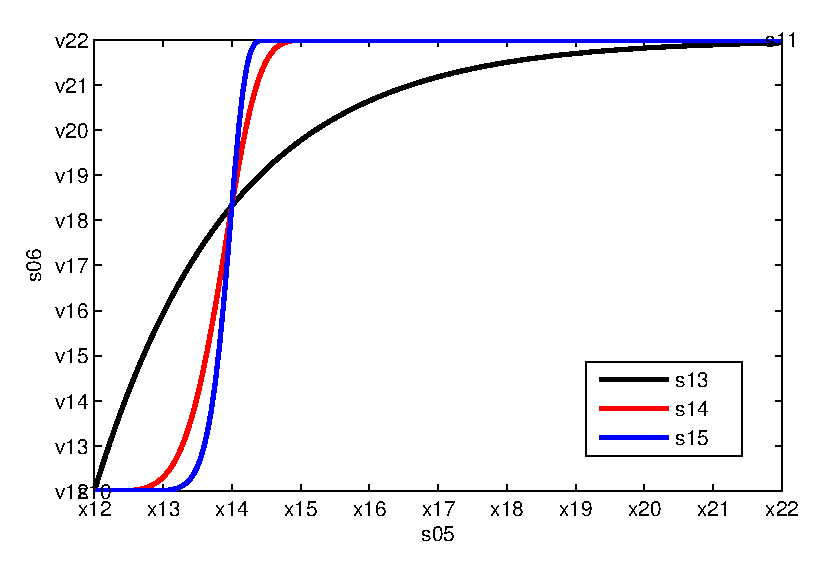
\includegraphics{./Images/Weibull.eps}}%
\end{psfrags}%
%
% End Weibull.tex
\end{document}
% See http://www.mathworks.de/matlabcentral/fileexchange/loadFile.do?objectId=4638
% for recent versions of laprint.m.
%
% created by:           LaPrint version 3.16 (13.9.2004)
% created on:           30-Dec-2013 09:44:00
% eps bounding box:     15 cm x 9.4415 cm
% comment:              
%
\begin{psfrags}%
\psfragscanon%
%
% text strings:
\psfrag{s05}[t][t]{\color[rgb]{0,0,0}\setlength{\tabcolsep}{0pt}\begin{tabular}{c}Applied Stress [Pa]\end{tabular}}%
\psfrag{s06}[b][b]{\color[rgb]{0,0,0}\setlength{\tabcolsep}{0pt}\begin{tabular}{c}Probability of Failure\end{tabular}}%
\psfrag{s10}[][]{\color[rgb]{0,0,0}\setlength{\tabcolsep}{0pt}\begin{tabular}{c} \end{tabular}}%
\psfrag{s11}[][]{\color[rgb]{0,0,0}\setlength{\tabcolsep}{0pt}\begin{tabular}{c} \end{tabular}}%
\psfrag{s12}[l][l]{\color[rgb]{0,0,0}m=10}%
\psfrag{s13}[l][l]{\color[rgb]{0,0,0}m=1}%
\psfrag{s14}[l][l]{\color[rgb]{0,0,0}m=5}%
\psfrag{s15}[l][l]{\color[rgb]{0,0,0}m=10}%
%
% xticklabels:
\psfrag{x01}[t][t]{0}%
\psfrag{x02}[t][t]{0.1}%
\psfrag{x03}[t][t]{0.2}%
\psfrag{x04}[t][t]{0.3}%
\psfrag{x05}[t][t]{0.4}%
\psfrag{x06}[t][t]{0.5}%
\psfrag{x07}[t][t]{0.6}%
\psfrag{x08}[t][t]{0.7}%
\psfrag{x09}[t][t]{0.8}%
\psfrag{x10}[t][t]{0.9}%
\psfrag{x11}[t][t]{1}%
\psfrag{x12}[t][t]{0}%
\psfrag{x13}[t][t]{1}%
\psfrag{x14}[t][t]{2}%
\psfrag{x15}[t][t]{3}%
\psfrag{x16}[t][t]{4}%
\psfrag{x17}[t][t]{5}%
\psfrag{x18}[t][t]{6}%
\psfrag{x19}[t][t]{7}%
\psfrag{x20}[t][t]{8}%
\psfrag{x21}[t][t]{9}%
\psfrag{x22}[t][t]{\shortstack{10\\$\times 10^{8}\ $}}%
%
% yticklabels:
\psfrag{v01}[r][r]{0}%
\psfrag{v02}[r][r]{0.1}%
\psfrag{v03}[r][r]{0.2}%
\psfrag{v04}[r][r]{0.3}%
\psfrag{v05}[r][r]{0.4}%
\psfrag{v06}[r][r]{0.5}%
\psfrag{v07}[r][r]{0.6}%
\psfrag{v08}[r][r]{0.7}%
\psfrag{v09}[r][r]{0.8}%
\psfrag{v10}[r][r]{0.9}%
\psfrag{v11}[r][r]{1}%
\psfrag{v12}[r][r]{0}%
\psfrag{v13}[r][r]{0.1}%
\psfrag{v14}[r][r]{0.2}%
\psfrag{v15}[r][r]{0.3}%
\psfrag{v16}[r][r]{0.4}%
\psfrag{v17}[r][r]{0.5}%
\psfrag{v18}[r][r]{0.6}%
\psfrag{v19}[r][r]{0.7}%
\psfrag{v20}[r][r]{0.8}%
\psfrag{v21}[r][r]{0.9}%
\psfrag{v22}[r][r]{1}%
%
% Figure:
\resizebox{9cm}{!}{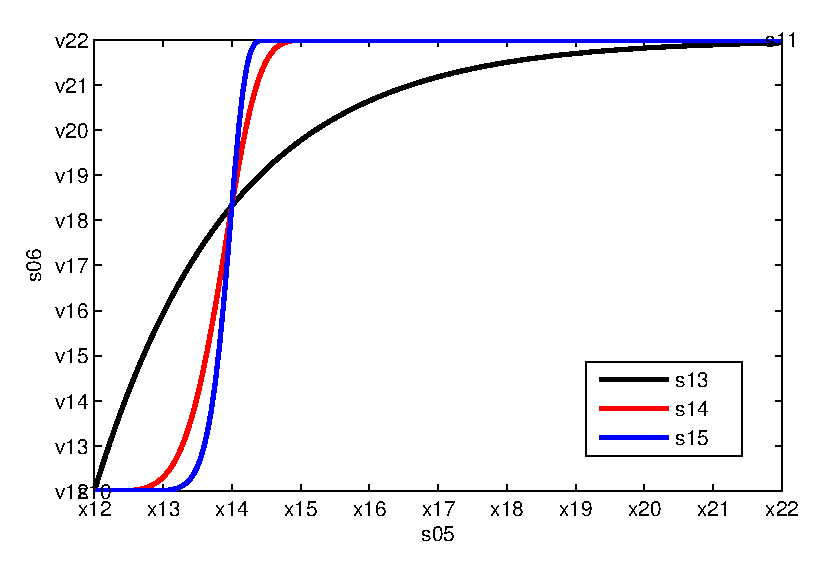
\includegraphics{./Images/Weibull.eps}}%
\end{psfrags}%
%
% End Weibull.tex
\end{document}
% See http://www.mathworks.de/matlabcentral/fileexchange/loadFile.do?objectId=4638
% for recent versions of laprint.m.
%
% created by:           LaPrint version 3.16 (13.9.2004)
% created on:           30-Dec-2013 09:44:00
% eps bounding box:     15 cm x 9.4415 cm
% comment:              
%
\begin{psfrags}%
\psfragscanon%
%
% text strings:
\psfrag{s05}[t][t]{\color[rgb]{0,0,0}\setlength{\tabcolsep}{0pt}\begin{tabular}{c}Applied Stress [Pa]\end{tabular}}%
\psfrag{s06}[b][b]{\color[rgb]{0,0,0}\setlength{\tabcolsep}{0pt}\begin{tabular}{c}Probability of Failure\end{tabular}}%
\psfrag{s10}[][]{\color[rgb]{0,0,0}\setlength{\tabcolsep}{0pt}\begin{tabular}{c} \end{tabular}}%
\psfrag{s11}[][]{\color[rgb]{0,0,0}\setlength{\tabcolsep}{0pt}\begin{tabular}{c} \end{tabular}}%
\psfrag{s12}[l][l]{\color[rgb]{0,0,0}m=10}%
\psfrag{s13}[l][l]{\color[rgb]{0,0,0}m=1}%
\psfrag{s14}[l][l]{\color[rgb]{0,0,0}m=5}%
\psfrag{s15}[l][l]{\color[rgb]{0,0,0}m=10}%
%
% xticklabels:
\psfrag{x01}[t][t]{0}%
\psfrag{x02}[t][t]{0.1}%
\psfrag{x03}[t][t]{0.2}%
\psfrag{x04}[t][t]{0.3}%
\psfrag{x05}[t][t]{0.4}%
\psfrag{x06}[t][t]{0.5}%
\psfrag{x07}[t][t]{0.6}%
\psfrag{x08}[t][t]{0.7}%
\psfrag{x09}[t][t]{0.8}%
\psfrag{x10}[t][t]{0.9}%
\psfrag{x11}[t][t]{1}%
\psfrag{x12}[t][t]{0}%
\psfrag{x13}[t][t]{1}%
\psfrag{x14}[t][t]{2}%
\psfrag{x15}[t][t]{3}%
\psfrag{x16}[t][t]{4}%
\psfrag{x17}[t][t]{5}%
\psfrag{x18}[t][t]{6}%
\psfrag{x19}[t][t]{7}%
\psfrag{x20}[t][t]{8}%
\psfrag{x21}[t][t]{9}%
\psfrag{x22}[t][t]{\shortstack{10\\$\times 10^{8}\ $}}%
%
% yticklabels:
\psfrag{v01}[r][r]{0}%
\psfrag{v02}[r][r]{0.1}%
\psfrag{v03}[r][r]{0.2}%
\psfrag{v04}[r][r]{0.3}%
\psfrag{v05}[r][r]{0.4}%
\psfrag{v06}[r][r]{0.5}%
\psfrag{v07}[r][r]{0.6}%
\psfrag{v08}[r][r]{0.7}%
\psfrag{v09}[r][r]{0.8}%
\psfrag{v10}[r][r]{0.9}%
\psfrag{v11}[r][r]{1}%
\psfrag{v12}[r][r]{0}%
\psfrag{v13}[r][r]{0.1}%
\psfrag{v14}[r][r]{0.2}%
\psfrag{v15}[r][r]{0.3}%
\psfrag{v16}[r][r]{0.4}%
\psfrag{v17}[r][r]{0.5}%
\psfrag{v18}[r][r]{0.6}%
\psfrag{v19}[r][r]{0.7}%
\psfrag{v20}[r][r]{0.8}%
\psfrag{v21}[r][r]{0.9}%
\psfrag{v22}[r][r]{1}%
%
% Figure:
\resizebox{9cm}{!}{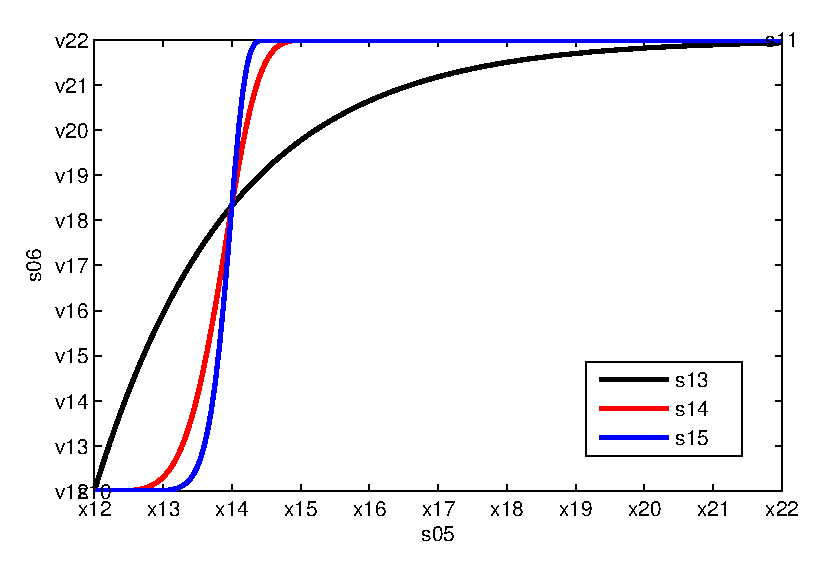
\includegraphics{./Images/Weibull.eps}}%
\end{psfrags}%
%
% End Weibull.tex

\label{fig:Weibull_CDF}
\end{figure}
\end{frame}

\begin{frame}{Weibull's Equation Properties}{Weibull's Equation Properties}
\begin{itemize}
\item considers size effects
\item considers only the uniaxial stress
\item computational simplicity
\item Phenomenological $\Longrightarrow$ not based on Fracture Mechanics Theory.
\end{itemize}
\end{frame}

\begin{frame}{Batdorf Approach}{Batdorf Approach}
\begin{eqnarray*}
P_f=1-exp\left[-\int_\Omega \int_V \int_{0}^{\sigma} dV \ d\Omega \ d\sigma_c \frac{dN\left(\sigma_c\right)}{d\sigma_c}\left(\frac{H\left(\sigma_e,\sigma_c\right)}{4 \pi}\right)\right]
\end{eqnarray*}
\begin{eqnarray*}
H\left(\sigma_e,\sigma_c\right) :\text{equals to 1 if } \sigma_e>\sigma_c
\end{eqnarray*}
\begin{eqnarray*}
N\left(\sigma_c\right) :\text{Number of cracks that has critical stress higher than } \sigma_c
\end{eqnarray*}
\begin{eqnarray*}
\sigma_c \text{: Critical stress}
\end{eqnarray*}
\begin{eqnarray*}
\Omega \text{: Area of unit sphere where } \sigma_{equavilent}>\sigma_c
\end{eqnarray*}
\end{frame}

\begin{frame}{Batdorf Approach}{Batdorf Approach}
Properties
\begin{itemize}
\item assumes random flaw orientation
\item consistent crack geometry
\end{itemize}
\end{frame}

\section{Applications}
\begin{frame}{Relation Between Statistics and Experiments}{Relation Between Statistics and Experiments}
Statistical models should base on real data from the experiments. Therefore, experiments should be done.
\end{frame}

\subsubsection{Experiments}
\begin{frame}{Experiments}{Experiment Properties}
\begin{itemize}
\item There are various type of experiments for the characterization of brittle material.
\item Experiments can be done both numerically and in laboratory conditions.
\end{itemize}
\end{frame}

\begin{frame}{Experiment types}{}
\begin{figure}
\centering
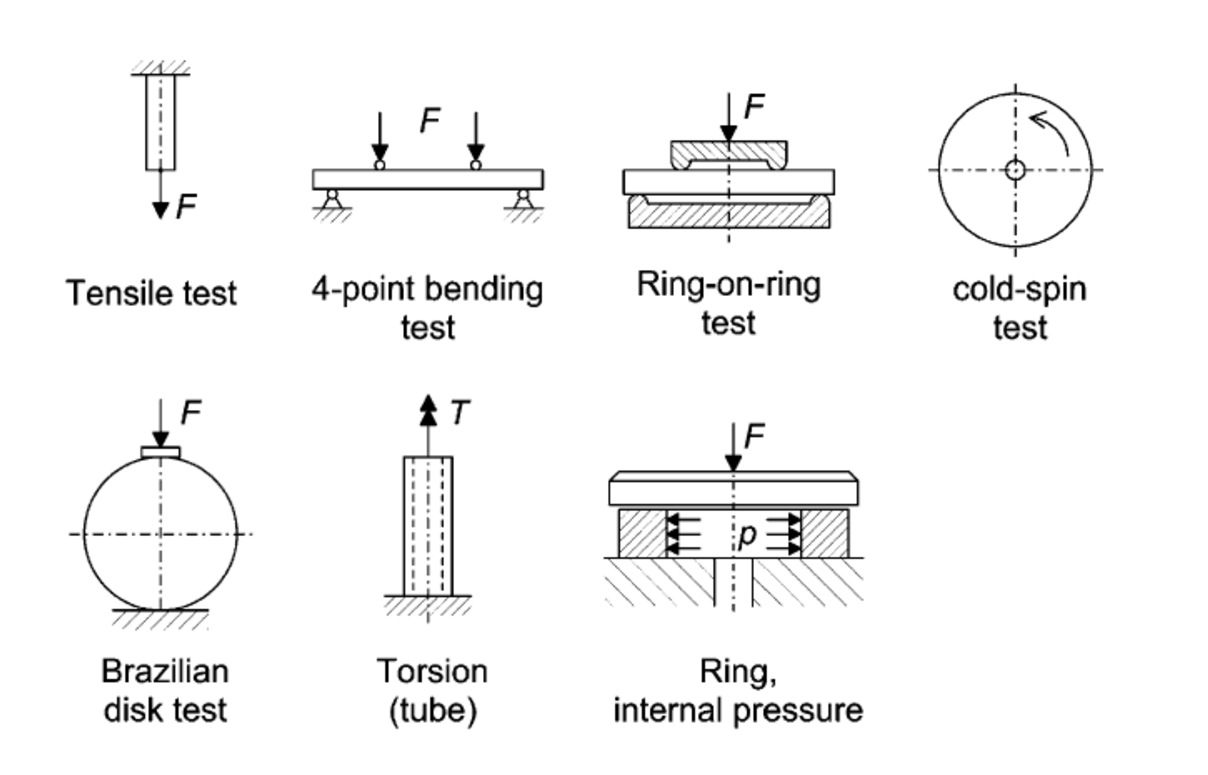
\includegraphics[width=0.7\linewidth]{./Images/experiments}
\label{fig:experiments}
\end{figure}
\emph{"The influence of failure criteria on strength prediction
of ceramic components", Patrick Scheunemann}
\end{frame}

\begin{frame}{Data collection and fit procedure for statistical representation}{}
\begin{itemize}
\item Collect $\sigma$ , probability of fracture data from specimens.
\item<2-> Determine $\sigma_0$ and $m$ in Weibull equation.
\end{itemize}
\end{frame}


\begin{frame}{Experiment types}
There is a computer code that is avaliable for statistical analysis of experiments.
\end{frame}

\begin{frame}{CARES}{An Interactive Code For Experiments and Curve Fitting fo Ceramics}
\begin{itemize}
\item developed at NASA
\item currently a commercial program
\item Abilities
\begin{itemize}
   \item Weibull parameter estimates
   \item Fatigue parameter estimates
   \item Multiaxial stress states
   \item Volume flaw  surface flaw analysis
   \item PIA, Weibull NSA, and Batdorf models
   \item Fast fracture reliability analysis
   \item Time-dependent reliability analysis (power law, Paris law, Walker law)
   \item Proof testing (PIA and Batdorf theories)
\end{itemize}\end{itemize}
\end{frame}

\begin{frame}{Applications}{Applications}
Aerospace Applications:
\begin{itemize}
    \item Mars Microprobe Aeroshell
    \item Small expendable turbojet
    \item APU Turbine wheel and nozzle
\end{itemize}
Automotive Applications:
\begin{itemize}
    \item Valves and engine components
    \item Turbine engine and components (scroll, combustor, rotor, insulation)
    \item Turbocharger wheel
\end{itemize}
Propulsion and Power Applications:
\begin{itemize}
    \item Turbine blade
\end{itemize}
Bioengineering Applications:
\begin{itemize}
    \item Dental Crowns
    \item Hip joint
\end{itemize}
\end{frame}




\section*{Summary}

\begin{frame}{Summary}

  % Keep the summary *very short*.
  \begin{itemize}
  \item
   Ceramic materials are brittle and they \alert{exhibit large variations} on fracture strength.
  \item
  	Brittleness makes \alert{use of statistical fracture is a must} for the prediction of failure.
   \item
  	Currently we have some tools that are usefull for \alert{use of statistical fracture is a must} for the prediction of failure.
  \end{itemize}
 
\end{frame}


\end{document}


